%% use
%% library(cacheSweave)
%% Sweave("unmarked.Rnw", driver = cacheSweaveDriver)


\documentclass[article,shortnames]{jss}
\usepackage{amsmath,amssymb}
\usepackage[utf8]{inputenc}
\usepackage{rotating}
%% need no \usepackage{Sweave.sty}


\DeclareMathOperator{\logit}{logit}
\DeclareMathOperator{\Bern}{Bernoulli}
\DeclareMathOperator{\Bin}{Binomial}
\DeclareMathOperator{\Poi}{Poisson}
\DeclareMathOperator{\MN}{Multinomial}

\newcommand{\um}{\pkg{unmarked}}
\newcommand{\rlang}{\proglang{R}}
\newcommand{\scovs}{\code{siteCovs}}
\newcommand{\ocovs}{\code{obsCovs}}

\author{Ian J. Fiske\\North Carolina State University \And
  Richard Chandler\\ USGS Patuxent Wildlife Research Center}
\title{\pkg{unmarked}:\\
  An \proglang{R} package for the Analysis of Wildlife Occurrence and Abundance Data}

\Plainauthor{Ian Fiske, Richard Chandler}
\Plaintitle{unmarked: An R Package for the Analysis of Wildlife
  Occurrence and Abundance Data}
\Shorttitle{\um: Analyze Wildlife Data in \proglang{R}}

\Abstract{Ecological research uses data collection techniques that are prone to 
substantial and unique types of measurement error to address scientific 
questions about species abundance and distribution.  These data collection 
schemes include a number of survey methods in which unmarked individuals are 
counted, or determined to be present, at numerous spatially-referenced sites.  
Examples include site occupancy sampling, repeated counts, distance sampling, 
removal sampling, and double observer sampling.  To appropriately analyze these 
data, hierarchical models have been developed that can separately model 
explanatory variables of both a latent abundance process and a conditional 
detection process.  Because these models have a straightforward interpretation 
paralleling how the data arose, they have recently gained immense popularity.  
The common hierarchical structure of these models is well-suited for a unified 
modeling interface.  The \proglang{R} package \pkg{unmarked} provides such a 
unified modeling framework, including tools for data exploration, model fitting, 
model criticism, post-hoc analysis, and model comparison.}

\Keywords{ecological, wildlife, hierarchical, occupancy, occurrence, distance, point count}
\Plainkeywords{ecological, wildlife, hierarchical, occupancy, occurrence, distance, point count}


\Address{
Ian Fiske\\
Department of Statistics\\
North Carolina State University\\
2311 Stinson Drive \\
Campus Box 8203 \\
Raleigh, NC 27695-8203 \\
E-mail: \email{ijfiske@ncsu.edu}

Richard Chandler \\   
USGS Patuxent Wildlife Research Center \\
Gabrielson Lab, Room 226 \\
12100 Beech Forest Rd. \\
Laurel, MD 20708 \\
E-mail: \email{rchandler@usgs.gov} 
}



\begin{document}


\section{Introduction}


\subsection{Imperfect detection in ecological research}

A fundamental goal of ecological research is to understand how environmental variables influence species abundance or occurrence.  Addressing these research questions is complicated by imperfect detection proability.  A species may go undetected when present for a variety of reasons including proximity to the observer, cryptic behavior, or camouflage.  To overcome these difficulties, ecologists have developed specialized methods to survey wildlife populations such as site occupancy sampling, repeated counts, distance sampling, removal sampling, and double observer sampling (see Section~\ref{sec:models-impl-unmark} for definitions).  Each of these sampling methods involves surveying a collection spatially-referenced `sites', which may be distinct habitat patches or arbitraryily-defined plots.  Observations are generated by a combination of (1) a \emph{state} process determining species abundance at each site and (2) a \emph{detection} process that yields observations conditional on the abundance.  Historically, ecologists ignored the detection process and fit standard generalized linear models to such data; however, failure to account for imperfect detection can yield grossly biased estimates of abundance or occurrence.  Therefore, the use of these specialized survey methods requires statistical models designed to appropriately account for both the state and observation processes. Recently devised hierarchical models provide a convenient means of accomodating both the state and detection processes.  Specifically,  these models regard site-specific abundance or occurence as a latent variable that may be impefectly observed.  This paper introduces \um, an \rlang\ package that provides a unified approach for fitting this class of hierarchical models.

\subsection[Scope and features of unmarked]{Scope and features of \pkg{unmarked}} 

\um\ provides tools to assist researchers with every step of the analysis process, including data manipulation and exploration, model fitting, post-hoc analysis, model criticism, and model selection.  Because of the multi-level structure of the data and models, covariate data can exist at both the state and detection level.  To succinctly describe these data, \um\ uses a new data type called the unmarkedFrame (Section~\ref{sec:data-requirements}).  \um\ provides functions that import data from various common formats and convert them into \um's data types.  Once imported, \um\ provides functions to summarize and subset these data in a manner familiar to users of \rlang's more common data structures such as vectors, matrices, and data frames. 

\um\ provides a growing list of model-fitting functions designed for specific sampling methods.  The fitting functions each find the maximum likelihood estimates of parameters from a particular model (Section~\ref{sec:fitting-models}) and return an object that can be easily manipulated.  Methods exist for performing numerous post-hoc analyses such as requesting linear combinations of parameters, back-transforming parameters to constrained scales, determining confidence intervals, and evaluating goodness of fit.  The model specification syntax of the fitting functions was designed to resemble the syntax of \rlang's common fitting functions such as \code{lm} for fitting linear models.

Although there is existing software for fitting some of these models \citep[e.g.,][for occupancy models]{Hines2002}, there are a number of advantages to a unified framework within \rlang.  Many researchers are already familiar with \rlang\ and use its powerful data manipulation and plotting capabilities.  Sometimes many species are analyzed in tandem, so that a common method of aggregating and post-processing of results is needed, a task easily accomplished in \rlang.  All of this is made much simpler by analyzing the data within \rlang, and using a single environment to complete all phases of the analysis is much less error-prone than switching between applications. Another important advantage of \um's approach is that researchers can easily simulate and analyze data within the same computational environment.  This work flow permits simulation studies for power analysis calculations or the effectiveness of future sampling designs.  An alternative approach for fitting these models is for researchers to program their own likelihood and maximize it within \rlang.  However, this requires that the researcher have well-developed programming abilities and also can require significant amount of overhead replicating code with minor tweaks for each new set of data.  \um\ provides a sufficiently flexible framework that many proposed models may be fit without extensive programming by the applied researcher.

In this paper, Section~\ref{sec:models-impl-unmark} gives a brief summary of many of the models \um\ is capable of fitting.  Section~\ref{sec:unmarked-usage} describes general \um\ usage aided by a running data example.

\section[Models implemented in unmarked]{Models implemented in \um}
\label{sec:models-impl-unmark}

The list of models implemented in \um\ continues to grow as new models are developed. Rather than describe each fitting function in detail, this section provides a summary of several of the most common sampling techniques and how \um\ can be used to model the resulting data. This section also introduces the syntax to illustrate how nicely it parallels the model structure, but full usage details are reserved for Section~\ref{sec:unmarked-usage}.

\begin{table} \small
%\begin{sidewaystable} \small
\begin{tabular}{cccc}
\hline
\textbf{Model} & \textbf{Fitting function} & \textbf{Data} & \textbf{Citation} \\ \hline
Occupancy & \code{occu} & unmarkedFrameOccu & \citep{MacKenzie2002} \\
Abundance from presence-absence & \code{occuRN}& unmarkedFrameOccu & \citep{Royle2003} \\
Repeated Counts &\code{pcount}& unmarkedFramePCount & \citep{Royle2004} \\
Distance-sampling &\code{distsamp}& unmarkedFrameDS & \citep{Royle2004b} \\
Multinomial Counts &\code{multinomPois}& unmarkedFrameMPois & \citep{Royle2004a} \\
Repeated Multinomial Counts &\code{gmultmix} & unmarkedFrameGMM & \citep{Royle2004a} \\
Colonization-extinction &\code{colext}& unmarkedMultFrame & \citep{MacKenzie2003} \\
Survival-recruitment & \code{pcountOpen} & unmarkedPCO & \citep{DailMadsen2011} \\
\hline
\end{tabular}
\caption{Models handled by unmarked along with their associated
  fitting functions (Section~\ref{sec:models-impl-unmark}) and data
  type (Section~\ref{sec:data-requirements}).}
\label{tab:models}
%\end{sidewaystable}
\end{table}

\subsection{Occurrence data} 
\label{sec:occ}

A popular estimand of interest in ecological research is the
proportion of sites that are used by the study species, called
occupancy probability.  Another related goal is to identify factors that are
associated with the changes in the probability of a site being
occupied.  To estimate these parameters, researchers employ
so-called occurrence sampling, whereby surveyors visit a sample of $R$
sites and record the binary response of species detection (1) or
non-detection (0) during $J_{i}$ visits to the $i$th site during a
`season' \citep{MacKenzie2002}.  The key assumptions that are made
when modelling these data are that the occupancy state at a site is
assumed to remain constant throughout the season and repeated visits at
a site are independent.

The repeated visits are necessary to obtain information about the
detection rate separate from the occupancy rate.  To describe these
data, we use the following hierarchical Bernoulli.  Let $\psi_i$ be
the probability of occupancy at site $i$.  And $p_{ij}$ is the
probability of detecting the species at site $i$ during the $j$th
survey occasion given that site $i$ is truly occupied.  More formally,
observations at site $i$ arise as
\begin{gather}
Z_i \sim \Bern(\psi_i) \text{\quad for $i=1,2,\dots,R$} \\
Y_{ij}|Z_i \sim \Bern(Z_i p_{ij})\text{\quad for $j=1,2,\dots,J_{i}$}
\end{gather}
where $Z_i$ is the partially observed occupancy state.

Variables that are suspected to be related to the occupancy state are 
modeled as
\begin{gather}
  \logit(\psi_i) = \mathbf x_i' \mathbf \beta,
\end{gather}
where $\mathbf x_i$ is a vector of observation covariates and $\mathbf \beta$
is a vector of their corresponding effect parameters.  Similarly, the
probability of detection can be modeled with
\begin{gather}
  \logit(p_{ij}) = \mathbf v_{ij}' \mathbf \alpha,
\end{gather}
where $\mathbf v_{ij}$ is a vector of survey-specific covariates and
$\mathbf \alpha$ is a vector of their corresponding effect parameters.

The likelihood then is

\begin{equation}
L(Y_{ij}| p,\phi) = 
 \prod_{i}^{R} \left\{
    \prod_{j}^{J} 
      \left(p^{Y_{ij}}(1-p)^{1-Y_{ij}}\right)
          \phi + I(Y_{i.}=0)(1-\phi) \right\} 
\end{equation}
                                                                                                            
Examples of site-specific covariates include habitat characteristics such as vegetation height. Observation-specific covariates could include time of day, date, wind speed, or other factors that might affect detection probability. 



\subsection{Repeated count data}
\label{sec:repeated-count-data}

Estimates of occupancy rate provide much less information about a
population than do abundance estimates. For instance, suppose the
average number of individuals per site decreases from 10 to 5 during
the course of a multi-season study. This dramatic population decline
would not be detected using occurence sampling.  One method to
estimate abundance is to repeatedly visit a sample of $R$ sites and
record the number of unique individuals observed at each site.
Similar assumptions are made as with occurrence data: (1) abundance at
a site remains constant during a season and (2) counts at a site are
independent.  \citet{Royle2004} presented the following hierarchical model for
repeated count data.  Let $N_i$ be the unobserved total number of
individuals using a site and define $Y_{ij}$ as the number of individuals observed
during the $j$th visit.  Then,
\begin{gather}
  N_i \sim f(\lambda_i, \theta) \text{\quad for $i=1,2,\dots,R$} \label{eq:pc2} \\
  Y_{ij}|N_{i} \sim \Bin(N_i, p_{ij})\text{\quad for $j=1,2,\dots,J_{i}$},
\end{gather}
where $\lambda_i$ is the abundance rate at site $i$ and $p_{ij}$ is
the detection probability during the $j$th visit to site $i$.  $f$ is
a discrete distribution with support restricted to $N_{i} \ge 0$ and
$\theta$ are extra parameters of $f$ other than the location
parameter, $\lambda_{i}$.  \um\ currently supports $f$ as Poisson or
negative binomial.  In the Poisson case, there is no $\theta$.  In the
negative binomial case, $\theta$ is a dispersion parameter, which is
useful when overdispersion is suspected.

\citet{Royle2004b} showed that in the case of the Poisson assumption, and if sites are independent, the integrated likelihood of $Y_{ij}$ is:

\begin{equation}
L(Y_{ij}| p,\lambda) = 
 \prod_{i}^{R} 
 \left\{ \sum_{N_{i}=max({\bf Y_i})}^{\infty}
          \left( \prod_{j}^{J} 
     \frac{N_{i!}}{ (N_{i}-Y_{ij})!} p^{Y_{ij}}(1-p)^{N_{i}-Y_{ij}} \right)
       \frac{e^{-\lambda} \lambda^N}{N!} \right\}
\end{equation}


As with the occupancy model, covariates may be included in either the
state (here, abundance) or detection levels, but abundance is modeled
through a log link to enforce it's positivity constraint.
\begin{gather}
  \log(\lambda_i) = \mathbf x_i' \mathbf \beta,
\end{gather}
where $\mathbf x_i$ is a vector of site-level covariates and $\mathbf \beta$
is a vector of their corresponding effect parameters.  Similarly, the
probability of detection can be modeled with
\begin{gather}
  \logit(p_{ij}) = \mathbf v_{ij}' \mathbf \alpha,
\end{gather}
where $\mathbf v_{ij}$ is a vector of observation-level covariates and
$\mathbf \alpha$ is a vector of their corresponding effect parameters.

     
\subsection{General multinomial-Poisson mixture model}
\label{sec:gener-mult-poiss}
Here we discuss a more general class of models that can be modified to fit a
variety of ecological sampling methods, the multinomial-Poisson model
\citep{Royle2004a}.  The general form of this model is
\begin{gather}
  N_i \sim \Poi(\lambda_i) \label{eq:mp2} \\
  \begin{pmatrix}
    \mathbf Y_i\\
    N_{i} - \sum_{j=1}^{J} Y_{ij}
  \end{pmatrix}
  \bigg| N_{i} \sim \MN\left(N_i, 
  \begin{pmatrix}
    \boldsymbol \pi_i \\
    \pi_{i}^{*}
  \end{pmatrix}\right),
\end{gather}
where $N_i$ is the latent abundance at site $i$ as with the point
count model, and $\boldsymbol \pi_i=(\pi_{i1},\pi_{i2},\dots,\pi_{iJ})'$ is
the vector of cell probabilities of observing responses in the $J$
possible categories, and $\mathbf Y_{i}$ is the $J$-vector of counts
that were actually observed.  In general, $\boldsymbol \pi_i$ is
determined by the specific sampling method and
$\sum_{j} \pi_{ij} \le 1$ because detection is imperfect and
$\pi_{i}^{*}=1 - \sum_{j} \pi_{ij}$ is the probability of the species
escaping detection at site $i$.  

Suppose that the sampling method yielded three observations at each cite. \citet{Royle2004a} demonstrated that if the observations ${\bf y}_i$ are independent when conditioned on local population size $N_i$ and $p_{it}$, the integrated likelihood of ${\bf y}_{i}$ is:
\begin{equation}
L({\bf y}_i| {\bf p},\lambda) = 
 \prod_{i=1}^{R} \left\{ 
  \sum_{N_{i}=0}^{\infty} \left(
 \frac{N_{i}!}{ y_{i1}! y_{i2}! y_{i3}! y_{i0}!}
  \pi_{1}^{y_{i1}}
  \pi_{2}^{y_{i2}}
  \pi_{3}^{y_{i3}}
  \pi^{*M_{i}- y_{i.}} \right)
 \frac{e^{-\lambda} \lambda^N}{N!} \right\}
\end{equation}

For multinomial-Poisson sampling methods, the actual observations are
an underlying categorical detection variable with $R \leq J$ levels so
that the $J$-dimensional $\mathbf Y_{i}$ is derived from the
$R$-dimensional raw counts in some sampling method-specific manner.
Thus, it is necessary to model the detection at the raw observation
level, denoted $p_{ik}$ for $k=1,2,\dots,R$ at site $i$.  Then we
derive the multinomial cell probabilities $\boldsymbol \pi_{i}$
through the sampling technique-specific relationship
$\pi_{ij}=g(p_{ik})$ where $p_{ik}$ is the underlying probability of
detection and $g$ is some sampling method-specific function.  

Thus, the only two requirements to adapt \um's general multinomial Poisson
modeling to a new sampling method is to specify $g$ and a binary 0-1
matrix that describes the mapping of elements of
$\mathbf p_{i} = (p_{i1},\dots,p_{iR})'$ to elements of
$\boldsymbol \pi_{i}$.  This mapping matrix, referred to in
\um\ as \code{obsToY}, is necessary to consistently clean
missing values from the data and relate observation-level covariates
with the responses.  The ($j$,$k$)th element of
\code{obsToY} is 1 only if $p_{ik}$ is involved in the computation of
$\pi_{ij}$.  The detection function $g$ is called \code{piFun} in \um.

Covariates may be included in either the
state (here, abundance) or detection levels, through $\mathbf p_{i}$
(not $\boldsymbol \pi_{i}$).
\begin{gather}
  \log(\lambda_i) = \mathbf x_i' \mathbf \beta,
\end{gather}
where $\mathbf x_i$ is a vector of site-level covariates and $\mathbf \beta$
is a vector of their corresponding effect parameters.  Similarly, the
probability of detection can be modeled with
\begin{gather}
  \logit(p_{ij}) = \mathbf v_{ij}' \mathbf \alpha,
\end{gather}
where $\mathbf v_{ij}$ is a vector of observation-level covariates and
$\mathbf \alpha$ is a vector of their corresponding effect parameters.

We now describe two common sampling methods that can be modeled
with the multinomial-Poisson model: removal sampling and double
observer sampling.  These two methods are included in \um, but
additional methods may easily be specified by the user with only the
\code{piFun} function and \code{obsToY} matrix.

\subsubsection{Removal sampling}

Popular in fisheries, removal sampling is implemented by visiting a
sample of $R$ sites $J$ times each and trapping and removing
individuals at each visit with the same effort.  Thus, $Y_{ij}$ is the
number of individuals captured at the $j$th visit for $j=1,2,\dots,J$.

Then, we can specify $g$ for removal sampling as follows.  The
probability of an individual at site $i$ being captured on the first
visit is $\pi_{i1} = p_{i1}$.  The probability of capture on the $j$th
visit is
\begin{equation}
  \pi_{ij} = \prod_{k=1}^{j-1}(1 - p_{ik})p_{ij},
\end{equation}
for $j=2,\dots,J$ and the probability of not being sampled is
\begin{equation}
  \pi_{i,J+1} = \prod_{j=1}^{J}(1-p_{ij})
\end{equation}
Or, equivalently,
\begin{equation}
  \mathbf \pi_i =
  \begin{pmatrix}
    p_{i1} \\
    (1-p_{i1})p_{i2} \\
    \vdots \\
    \prod_{j=1}^J(1-p_{ij})p_{iJ}
  \end{pmatrix}
\end{equation}
Thus, the mapping matrix is an $J \times R$ upper triangular matrix with ones in
the upper triangle,
\begin{equation}
  \begin{pmatrix}
    1 & 1 & \dots & 1 \\
    0 & 1 & \dots & 1 \\
    \vdots & & \ddots & \vdots \\
    0 & 0 & \dots  & 1
  \end{pmatrix}
\end{equation}


\subsubsection{Double observer sampling}
\label{sec:double-observ-sampl}

Double observer sampling collects data by a team of two surveyors
simultaneously visiting a site.  They each collect lists of identified
animals.  Thus the counts in the three cells of $\mathbf Y_i$
correspond to the numbers of individuals seen by observer one,
observer two, or both.  Thus, for double observer sampling, $g$ is
defined as follows.
\begin{equation}
  \mathbf \pi_i =
  \begin{pmatrix}
    p_{i1}(1-p_{i2}) \\
    (1-p_{i1})p_{i2} \\
    p_{i1}p_{i2} \\
    (1-p_{i1})(1-p_{i2}).
  \end{pmatrix}
\end{equation}
The \code{obsToY} mapping matrix for double observer sampling is the
following $3 \times 2$ matrix.
\begin{equation}
  \begin{pmatrix}
    1 & 0 \\
    0 & 1 \\
    1 & 1 
  \end{pmatrix}
\end{equation}


\subsection{Colonization-extinction data}

Sometimes the study objective is to understand the evolution of
the occupancy state over time.  To obtain such information researchers conduct 
repeated occupancy studies (see Section~\ref{sec:occ}) at the same sample of 
sites over consecutive seasons \citep{MacKenzie2003}.  They then seek to estimate
probabilities of colonization ($\gamma_{it}$) and extinction
($\epsilon_{it}$), where colonization is the change of an unoccupied
site to occupied and extinction if the change of an occupied site to
unoccupied.  If the occupancy status is assumed to evolve according to
a Markov process, then a 2-state finite hidden Markov model describes
these data.  Let $Y_{itj}$ denote the observed animal occurrence
status at visit $j$ during season $t$ to site $i$.  Then
\begin{gather}
  Z_{i1} \sim \Bern(\psi) \\
  Z_{it} \sim
  \begin{cases}
    \Bern(\gamma_{i(t-1)}) & \text{if $Z_{i(t-1)} = 0$} \\
    \Bern(1-\epsilon_{i(t-1)}) & \text{if $Z_{i(t-1)} = 1$}
  \end{cases}, \\
  \text{for $t=2,3,\dots,T$} \notag \\
  Y_{itj} | Z_{it} \sim \Bern(Z_{it} p_{itj})
\end{gather}


The likelihood of this model is

\begin{equation}
L(Y_{ijt}| p,\phi,\epsilon,\gamma) = 
 \prod_{i}^{R} \left\{
    \Psi_0 \prod_{t}^{T-1} 
      \Phi_t \left(p^{Y_{ijt}}(1-p)^{1-Y_{ijt}}\right)
          \Psi_t + I({\bf Y_{it}}=0)(1-\Psi_t) \right\} 
\end{equation}
 


\section[unmarked usage]{\pkg{unmarked} usage}
\label{sec:unmarked-usage}

\um\ provides
data structures, fitting syntax, and post-processing that form a
cohesive framework for site-based ecological data analysis.  In order
to achieve these goals, \um\ uses the S4 class system
\citep{Chambers2008}. As \rlang's most modern system of class-based
programming, S4 allows customization of functions, referred to as
methods, to specific object classes and superclasses. For example,
when the generic \code{predict} method is called with any \um\ model
fit object as an argument, the actual \code{predict} implementation
depends on the specific model that was fit.  Use of class-based
programming can provide more reliable and maintainable software while
also making the program more user-friendly \citep{Chambers2008}.


\subsection{Preparing data}
\label{sec:data-requirements}

\um\ uses a custom S4 data structure called the unmarkedFrame
to store all data related to a sampling survey.  Although this at
first appears to add an extra layer of work for the user, there are
several reasons for this design choice.  The multilevel structure of
the models means that standard rectangular data structures such as data
frames or matrices are not suitable for storing the data.  For
example, covariates might have been measured separately at the site
level and at the visit level.  Furthermore, the length of the response
vector $\mathbf Y_{i}$ at site $i$ might differ from the number of
observations at the site as in the multinomial Poisson model.  Aside
from these technical reasons, \citet{Gentleman2009} pointed out that
the use of such portable custom data objects can simplify future
reference to previous analyses, an often neglected aspect of research.
Repeated fitting calls using the same set of data require less code
repetition if all data is contained in a single object.  Finally,
calls to fitting functions have a cleaner appearance with a more
obvious purpose when the call is not buried in data arguments.  The
parent data class is called an unmarkedFrame and each \um\
fitting function has its own data type that extends the
unmarkedFrame.  Thus, the first step when using \um\ is to
import data into the proper type of unmarkedFrame.  To ease
this step, \um\ includes several helper functions to automatically
convert data into an unmarkedFrame: \code{csvToUMF} which
imports data directly from a comma-separated value text file,
\code{formatWide} and \code{formatLong} which convert data from data
frames, and the family of unmarkedFrame constructor functions.

An unmarkedFrame object contains components referred to as slots, which hold the data and metadata. All unmarkedFrame objects contain a slot for the observation matrix \code{y}, a data frame of site-level covariates \code{siteCovs}, and a
data frame of observation-level covariates \code{obsCovs}.  The
\code{y} matrix is the only required unmarkedFrame slot.  \code{y} is
an $M \times J$ matrix with the $i$th row containing the
$J$-dimensional $\mathbf y_i$.  If $J_{i} \le J$, then any number of
elements of $\mathbf y_{i}$ can take the value \code{NA} to denote
this.  \code{siteCovs} is an $M$-row data frame with a column for each
site-level covariate.  \code{obsCovs} is an $RJ$-row data frame with a
column for each observation-level covariate.  Thus each row of
\code{obsCovs} corresponds to a particular observation, with the order
corresponding to site varying slower and observation within site
varying faster.  Both \scovs\ and \ocovs\ can contain \code{NA}
values corresponding to unbalanced data collection.  If any terms in the model
specification are missing for that observation, \um\
automatically removes observations.  \um\ provides
constructor functions to make creating unmarkedFrames straightforward.
For each specific data type, specific types of unmarkedFrames extend
the basic unmarkedFrame to handle model-specific nuances.

\subsubsection{Importing repeated count data}

Here is an example of creating an unmarkedFrame for point count data
(Section~\ref{sec:repeated-count-data}).
from a list a matrix of observations, a data frame of site-level
covariates, and a list of matrices of observation-level covariates.

First, load the included data set of Mallard duck point counts from
\citet{Kery2005} and visually inspect the point count matrix, which is
already in the same format as the \code{y} slot of an unmarkedFrame.

\begin{Schunk}
\begin{Sinput}
> library(unmarked)
> data(mallard)
\end{Sinput}
\end{Schunk}

Loading the mallard data makes three objects availble within the \rlang workspace. The response matrix \code{mallard.y} is formatted such that each row is a site and each columnn corresponds to a survey occasion.  The site-level covariates are column vectors in the \code{mallard.site} data.frame, which has R rows. The observation-level covariates are a list object with separate $R \times J$ matrices for each observation-level covariate.  The unmarkedFrame constructors can accept \ocovs\ in this list format or as a data frame in the format described above.

The following call to \code{unmarkedFramePCount} function creates an unmarkedFramePCount object, which is the specific type of unmarkedFrame for point count data.

\begin{Schunk}
\begin{Sinput}
> mallardUMF <- unmarkedFramePCount(y = mallard.y, siteCovs = mallard.site, 
+     obsCovs = mallard.obs)
\end{Sinput}
\end{Schunk}

Printing unmarkedFrames shows them as data frames to make it easier to verify that the data were converted correctly. Here we show the first five rows only. 

\begin{Schunk}
\begin{Sinput}
> head(mallardUMF, 5)
\end{Sinput}
\begin{Soutput}
Data frame representation of unmarkedFrame object.
  y.1 y.2 y.3   elev length forest ivel.1 ivel.2 ivel.3 date.1 date.2
1   0   0   0 -1.173  0.801 -1.156 -0.506 -0.506 -0.506 -1.761  0.310
2   0   0   0 -1.127  0.115 -0.501 -0.934 -0.991 -1.162 -2.904 -1.047
3   3   2   1 -0.198 -0.479 -0.101 -1.136 -1.339 -1.610 -1.690 -0.476
4   0   0   0 -0.105  0.315  0.008 -0.819 -0.927 -1.197 -2.190 -0.690
5   3   0   3 -1.034 -1.102 -1.193  0.638  0.880  1.042 -1.833  0.167
  date.3
1  1.381
2  0.596
3  1.453
4  1.239
5  1.381
\end{Soutput}
\end{Schunk}

The site-specific covariates are elevation (elev), transect length (length), and the proportion of forest covering the site. The two observation covariates are a measure of survey effort (ivel) and the date of the survey (date). We can also check data contents with a quick summary.

\begin{Schunk}
\begin{Sinput}
> summary(mallardUMF)
\end{Sinput}
\begin{Soutput}
unmarkedFrame Object

239 sites
Maximum number of observations per site: 3 
Mean number of observations per site: 2.76 
Sites with at least one detection: 40 

Tabulation of y observations:
   0    1    2    3    4    7   10   12 <NA> 
 576   54   11    9    6    1    1    1   58 

Site-level covariates:
      elev                length               forest          
 Min.   :-1.436e+00   Min.   :-4.945e+00   Min.   :-1.265e+00  
 1st Qu.:-9.565e-01   1st Qu.:-5.630e-01   1st Qu.:-9.560e-01  
 Median :-1.980e-01   Median : 4.500e-02   Median :-6.500e-02  
 Mean   :-4.603e-05   Mean   :-2.929e-05   Mean   : 6.695e-05  
 3rd Qu.: 9.940e-01   3rd Qu.: 6.260e-01   3rd Qu.: 7.900e-01  
 Max.   : 2.434e+00   Max.   : 2.255e+00   Max.   : 2.299e+00  

Observation-level covariates:
      ivel                 date           
 Min.   :-1.753e+00   Min.   :-2.904e+00  
 1st Qu.:-6.660e-01   1st Qu.:-1.119e+00  
 Median :-1.390e-01   Median :-1.190e-01  
 Mean   : 1.504e-05   Mean   : 7.259e-05  
 3rd Qu.: 5.490e-01   3rd Qu.: 1.310e+00  
 Max.   : 5.980e+00   Max.   : 3.810e+00  
 NA's   : 5.200e+01   NA's   : 4.200e+01  
\end{Soutput}
\end{Schunk}

The summary reveals that only 40 sites have at least one detection -- these data are in fact very sparse as is commonplace in ecological statistics. The tabulation of y observations provides additional evidence of sparse counts, with no mallards being detected at 576 of the surveys. The 58 NA values correspond to missing data. 


\subsubsection{Importing removal sampling data}

To illustrate the slightly different syntax for removal sampling data example, we will import data from a removal survey of Ovenbirds described by \citet{Royle2004a}.  The data consist of a list with a matrix \code{data} containing the removal counts for 4 visits and a data frame called \code{covariates} containing site-level covariates information.

\begin{Schunk}
\begin{Sinput}
> data(ovendata)
\end{Sinput}
\end{Schunk}

Each row of the response data corresponds to a site, and each column is a removal occasion. Thus, it is evident that ovenbirds were detected at three of the first ten sites and no new birds were detected after the first removal occasion.  The only additional specification required when importing removal data is to
specify the particular type of multinomial-Poisson data as
\code{removal} via the \code{type} argument.

\begin{Schunk}
\begin{Sinput}
> scaled.covs <- as.data.frame(scale(ovendata.list$covariates[, 
+     -1]))
> ovenFrame <- unmarkedFrameMPois(ovendata.list$data, siteCovs = scaled.covs, 
+     type = "removal")
> summary(ovenFrame)
\end{Sinput}
\begin{Soutput}
unmarkedFrame Object

70 sites
Maximum number of observations per site: 4 
Mean number of observations per site: 4 
Sites with at least one detection: 44 

Tabulation of y observations:
   0    1    2    3 <NA> 
 218   49   11    2    0 

Site-level covariates:
      ufp                  trba           
 Min.   :-1.471e+00   Min.   :-2.010e+00  
 1st Qu.:-7.408e-01   1st Qu.:-6.931e-01  
 Median :-2.535e-01   Median :-1.287e-01  
 Mean   : 1.351e-17   Mean   :-2.531e-16  
 3rd Qu.: 9.844e-01   3rd Qu.: 7.178e-01  
 Max.   : 2.344e+00   Max.   : 2.881e+00  
\end{Soutput}
\end{Schunk}


\subsection{Fitting models}
\label{sec:fitting-models}

As introduced in Section~\ref{sec:models-impl-unmark}, each model has a
corresponding fitting function.  For example, to fit a repeated count
model, we call \code{pcount}.  Table~\ref{tab:models} provides a
summary of all models that \um\ currently fits.  With the exception of colext,
all fitting functions use a double right-hand sided formula syntax that expresses the hierarchical model and data structures.  Specifically, covariates affecting the detection process are specified following the first tilda, and covariates of the state process follow the second tilda. No left-hand side of the formula is specified because the unmarkedFrame defines the response variable
uniquely as the \code{y} slot.

\subsubsection{Fitting a repeated count model}

Continuing the Mallard example, the following call to \code{pcount} fits an binomaial-Poisson mixture model (Section~\ref{sec:repeated-count-data}).  The following code specifies that detection probability $p$ should be modeled by day of year, including a quadratic term.  We also wish to model abundance using elevation and proportion of area forested.  As described in Section~\ref{sec:repeated-count-data}, covariates of detection are on the logit-scale and covariates of abundance are on the log scale for the point count model.

\begin{Schunk}
\begin{Sinput}
> fm.mallard.1 <- pcount(~date + I(date^2) ~ elev + forest, 
+     data = mallardUMF)
> fm.mallard.1
\end{Sinput}
\begin{Soutput}
Call:
pcount(formula = ~date + I(date^2) ~ elev + forest, data = mallardUMF)

Abundance:
            Estimate    SE     z  P(>|z|)
(Intercept)   -1.853 0.236 -7.87 3.62e-15
elev          -1.232 0.234 -5.27 1.36e-07
forest        -0.756 0.165 -4.60 4.32e-06

Detection:
            Estimate     SE       z P(>|z|)
(Intercept)   0.3071 0.2149  1.4290 0.15301
date         -0.4091 0.1482 -2.7612 0.00576
I(date^2)    -0.0077 0.0853 -0.0903 0.92801

AIC: 521.2001 
\end{Soutput}
\end{Schunk}

%%%% This interpretation comes before model results are presented
This initial fit suggests that Mallard abundance decreases with
increasing elevation and forest.  It also looks like a linear model
might suffice for the detection model, so we subsequently fit the
linear detection model.


\begin{Schunk}
\begin{Sinput}
> fm.mallard.2 <- pcount(~date ~ elev + forest, data = mallardUMF)
> fm.mallard.2
\end{Sinput}
\begin{Soutput}
Call:
pcount(formula = ~date ~ elev + forest, data = mallardUMF)

Abundance:
            Estimate    SE     z  P(>|z|)
(Intercept)   -1.857 0.232 -7.99 1.37e-15
elev          -1.236 0.230 -5.38 7.59e-08
forest        -0.756 0.164 -4.60 4.23e-06

Detection:
            Estimate    SE     z  P(>|z|)
(Intercept)    0.298 0.188  1.58 0.113983
date          -0.401 0.114 -3.51 0.000449

AIC: 519.2081 
\end{Soutput}
\end{Schunk}

This seems to be a better model according to both the Wald p-value and
AIC.  Thus detection appears to decrease during the course of a year.



\subsubsection{Fitting a multinomial-Poisson model}

Here we demonstrate fitting a multinomial-Poisson model to removal sampling 
data.  The Ovenbird data has no observation-level covariates, so detection
probability is assumed constant across visits.  It is not necessary
to specify that removal sampling was used when fitting the model
because this information is already stored in the \code{ovenFrame} data.
We model the abundance with understory forest coverage (\code{ufp})
and average basal tree area (\code{trba}).

\begin{Schunk}
\begin{Sinput}
> fm.oven.1 <- multinomPois(~1 ~ ufp + trba, ovenFrame)
> fm.oven.1
\end{Sinput}
\begin{Soutput}
Call:
multinomPois(formula = ~1 ~ ufp + trba, data = ovenFrame)

Abundance:
            Estimate    SE      z P(>|z|)
(Intercept)    0.102 0.119  0.864   0.388
ufp            0.100 0.126  0.794   0.427
trba          -0.171 0.135 -1.262   0.207

Detection:
 Estimate    SE    z P(>|z|)
    0.288 0.233 1.24   0.217

AIC: 326.1387 
\end{Soutput}
\end{Schunk}

\subsection{Examining model fits}
\label{sec:examining-model-fits}

Objects returned by \um's fitting functions also make use of the S4
class system.  All model fit objects belong to the unmarkedFit parent
class.  Thus, common operations such as extracting coefficient
estimates, covariance matrices for estimates, and confidence intervals
have been adapted to behave similar to \rlang's base functions.


For example, we can extract estimated coefficients either from the
entire model, or from the state or detection levels by specifying the
\code{type} argument.

\begin{Schunk}
\begin{Sinput}
> coef(fm.mallard.2)
\end{Sinput}
\begin{Soutput}
   lam(Int)   lam(elev) lam(forest)      p(Int)     p(date) 
 -1.8565048  -1.2355497  -0.7555178   0.2977558  -0.4006066 
\end{Soutput}
\begin{Sinput}
> coef(fm.mallard.2, type = "state")
\end{Sinput}
\begin{Soutput}
   lam(Int)   lam(elev) lam(forest) 
 -1.8565048  -1.2355497  -0.7555178 
\end{Soutput}
\end{Schunk}

To check which types are available for a model, use the \code{names} method.

\begin{Schunk}
\begin{Sinput}
> names(fm.mallard.2)
\end{Sinput}
\begin{Soutput}
[1] "state" "det"  
\end{Soutput}
\end{Schunk}

Similarly, the \code{vcov} function extracts the covariance matrix of
the estimates, using the observed Fisher information by default.

\begin{Schunk}
\begin{Sinput}
> vcov(fm.mallard.2)
\end{Sinput}
\begin{Soutput}
                lam(Int)    lam(elev)   lam(forest)       p(Int)
lam(Int)     0.054013257  0.040740133  0.0080777484 -0.006188545
lam(elev)    0.040740133  0.052810074 -0.0084624468 -0.001751201
lam(forest)  0.008077748 -0.008462447  0.0269780875  0.001779971
p(Int)      -0.006188545 -0.001751201  0.0017799714  0.035490236
p(date)     -0.001785422 -0.003393574  0.0005126907  0.003448530
                  p(date)
lam(Int)    -0.0017854217
lam(elev)   -0.0033935742
lam(forest)  0.0005126907
p(Int)       0.0034485301
p(date)      0.0130286462
\end{Soutput}
\end{Schunk}

\code{vcov} also accepts a \code{type} argument.

\begin{Schunk}
\begin{Sinput}
> vcov(fm.mallard.2, type = "state")
\end{Sinput}
\begin{Soutput}
               lam(Int)    lam(elev)  lam(forest)
lam(Int)    0.054013257  0.040740133  0.008077748
lam(elev)   0.040740133  0.052810074 -0.008462447
lam(forest) 0.008077748 -0.008462447  0.026978088
\end{Soutput}
\end{Schunk}

\um\ also provides an associated helper function \code{SE} to return
standard errors from the square root of the diagonal of these
covariance matrices.

\begin{Schunk}
\begin{Sinput}
> SE(fm.mallard.2)
\end{Sinput}
\begin{Soutput}
   lam(Int)   lam(elev) lam(forest)      p(Int)     p(date) 
  0.2324075   0.2298044   0.1642501   0.1883885   0.1141431 
\end{Soutput}
\begin{Sinput}
> SE(fm.mallard.2, type = "state")
\end{Sinput}
\begin{Soutput}
   lam(Int)   lam(elev) lam(forest) 
  0.2324075   0.2298044   0.1642501 
\end{Soutput}
\end{Schunk}

Nonparametric bootstrapping can also be used to estimate the
covariance matrix. \um\ implements a two-stage bootstrap in which the
sites are first drawn with replacement, and then within each site, the
observations are drawn with replacement.  First, bootstrap draws must
be taken using the \code{nonparboot}.  \code{nonparboot} returns a new
version of the unmarkedFit object with additional bootstrap sampling
information.  Thus, this new fit must be stored, either in a new fit
object or the same one, and then subsequently queried for bootstrap
summaries.  In the following, bootstrapping can be quite slow.  For
these examples, we illustrate with the removal sampling data simply
because computations are much faster.  However, bootstrapping is
available for any of the models that \um\ fits.

\begin{Schunk}
\begin{Sinput}
> set.seed(1234)
> fm.oven.1 <- nonparboot(fm.oven.1, B = 100)
\end{Sinput}
\end{Schunk}

\begin{Schunk}
\begin{Sinput}
> SE(fm.oven.1, type = "state")
\end{Sinput}
\begin{Soutput}
 lambda(Int)  lambda(ufp) lambda(trba) 
   0.1185431    0.1262615    0.1353444 
\end{Soutput}
\begin{Sinput}
> SE(fm.oven.1, type = "state", method = "nonparboot")
\end{Sinput}
\begin{Soutput}
 lambda(Int)  lambda(ufp) lambda(trba) 
   0.1256949    0.1156153    0.1197142 
\end{Soutput}
\end{Schunk}

It looks like bootstrapping and asymptotic standard errors are close.
The summary now states the number of bootstrap samples.

\begin{Schunk}
\begin{Sinput}
> summary(fm.oven.1)
\end{Sinput}
\begin{Soutput}
Call:
multinomPois(formula = ~1 ~ ufp + trba, data = ovenFrame)

Abundance (log-scale):
            Estimate    SE      z P(>|z|)
(Intercept)    0.102 0.119  0.864   0.388
ufp            0.100 0.126  0.794   0.427
trba          -0.171 0.135 -1.262   0.207

Detection (logit-scale):
 Estimate    SE    z P(>|z|)
    0.288 0.233 1.24   0.217

AIC: 326.1387 
Number of sites: 70
optim convergence code: 0
optim iterations: 33 
Bootstrap iterations: 100 
\end{Soutput}
\end{Schunk}

Additional bootstrap samples can be drawn by calling \code{nonparboot} again.
\begin{Schunk}
\begin{Sinput}
> fm.oven.1 <- nonparboot(fm.oven.1, B = 100)
\end{Sinput}
\end{Schunk}

Confidence intervals can be requested for the coefficients at either
stage of the model.  By default, the asymptotic normal approximation
is used.

\begin{Schunk}
\begin{Sinput}
> confint(fm.oven.1, type = "state", level = 0.95)
\end{Sinput}
\begin{Soutput}
                  0.025      0.975
lambda(Int)  -0.1299722 0.33470834
lambda(ufp)  -0.1471741 0.34776195
lambda(trba) -0.4361311 0.09440937
\end{Soutput}
\end{Schunk}

Profile confidence intervals are also available upon request.  This
can take some time, however, because for each parameter, a nested
optimization within a root-finding algorithm is being used to find the
profile limit.

\begin{Schunk}
\begin{Sinput}
> ci <- confint(fm.oven.1, type = "state", level = 0.95, 
+     method = "profile")
\end{Sinput}
\begin{Soutput}
Profiling parameter 1 of 3 ... done.
Profiling parameter 2 of 3 ... done.
Profiling parameter 3 of 3 ... done.
\end{Soutput}
\end{Schunk}
\begin{Schunk}
\begin{Sinput}
> ci
\end{Sinput}
\begin{Soutput}
                  0.025      0.975
lambda(Int)  -0.1390786 0.32676614
lambda(ufp)  -0.1477724 0.34811770
lambda(trba) -0.4368444 0.09469605
\end{Soutput}
\end{Schunk}

The profile confidence intervals and normal approximations are quite
similar here.

\subsubsection{Linear combinations of estimates}

Often, meaningful hypotheses can be addressed by estimating linear
combinations of coefficient estimates.  Linear combinations of coefficient
estimates can be requested with \code{linearComb}.

Continuing the Ovenbird example, the following code estimates the
log-abundance rate for a site with \code{ufp = 0.5} and \code{trba
  = 0}.

\begin{Schunk}
\begin{Sinput}
> (lc <- linearComb(fm.oven.1, type = "state", coefficients = c(1, 
+     0.5, 0)))
\end{Sinput}
\begin{Soutput}
Linear combination(s) of Abundance estimate(s)

 Estimate    SE (Intercept) ufp trba
    0.153 0.130           1 0.5    0
\end{Soutput}
\end{Schunk}

Multiple sets of coefficients may be supplied as a matrix.  The
following code requests the estimated log-abundance for sites with
\code{ufp = 0.5} and \code{trba = 1}.

\begin{Schunk}
\begin{Sinput}
> (lc <- linearComb(fm.oven.1, type = "state", coefficients = matrix(c(1, 
+     0.5, 0, 1, 1, 0), 2, 3, byrow = TRUE)))
\end{Sinput}
\begin{Soutput}
Linear combination(s) of Abundance estimate(s)

  Estimate    SE (Intercept) ufp trba
1    0.153 0.130           1 0.5    0
2    0.203 0.166           1 1.0    0
\end{Soutput}
\end{Schunk}

Standard errors and confidence intervals are also available for linear
combinations of parameters.  By requesting nonparametric bootstrapped
standard errors, \um\ uses the samples that were drawn earlier.

\begin{Schunk}
\begin{Sinput}
> SE(lc)
\end{Sinput}
\begin{Soutput}
[1] 0.1296526 0.1659460
\end{Soutput}
\begin{Sinput}
> SE(lc, method = "nonparboot")
\end{Sinput}
\begin{Soutput}
[1] 0.1354092 0.1659877
\end{Soutput}
\begin{Sinput}
> confint(lc)
\end{Sinput}
\begin{Soutput}
       0.025     0.975
1 -0.1015993 0.4066294
2 -0.1225862 0.5279102
\end{Soutput}
\end{Schunk}

\subsubsection{Back-transforming linear combinations of coefficients}

Estimates of linear combination back-transformed to the native scale
are likely to be more interesting than the direct linear combinations.
For example, the logistic transformation is applied to estimates of
detection rates, resulting in a probability bound between 0 and
1. This is accomplished with the \code{backTransform}.  Standard
errors of back-transformed estimates are estimated using the delta
method.  Confidence intervals are estimated by back-transforming the
confidence interval of the original linear combination.

\begin{Schunk}
\begin{Sinput}
> (btlc <- backTransform(lc))
\end{Sinput}
\begin{Soutput}
Backtransformed linear combination(s) of Abundance estimate(s)

  Estimate    SE LinComb (Intercept) ufp trba
1     1.16 0.151   0.153           1 0.5    0
2     1.22 0.203   0.203           1 1.0    0

Transformation: exp 
\end{Soutput}
\begin{Sinput}
> SE(btlc)
\end{Sinput}
\begin{Soutput}
[1] 0.1510141 0.2032272
\end{Soutput}
\begin{Sinput}
> SE(btlc, method = "nonparboot")
\end{Sinput}
\begin{Soutput}
[1] 0.1577193 0.2032782
\end{Soutput}
\begin{Sinput}
> confint(btlc)
\end{Sinput}
\begin{Soutput}
      0.025    0.975
1 0.9033915 1.501747
2 0.8846296 1.695386
\end{Soutput}
\end{Schunk}


\subsubsection{Model selection}

\pkg{unmarked} performs simple AIC-based model selection for structured lists of unmarkedFit objects.  To demonstrate, we fit a few more models to the Ovenbird
removal data, including all an interaction model, two models with
single predictors, and a null model with no predictors.

\begin{Schunk}
\begin{Sinput}
> fm.oven.2 <- update(fm.oven.1, formula = ~1 ~ ufp * trba)
> fm.oven.3 <- update(fm.oven.1, formula = ~1 ~ ufp)
> fm.oven.4 <- update(fm.oven.1, formula = ~1 ~ trba)
> fm.oven.5 <- update(fm.oven.1, formula = ~1 ~ 1)
\end{Sinput}
\end{Schunk}

Now, we can organize the fitted models with the \code{fitList} function and
the use the \code{modSel} method to rank the models by AIC.



\begin{Schunk}
\begin{Sinput}
> fmList <- fitList(Global = fm.oven.2, additive = fm.oven.1, 
+     ufp = fm.oven.3, trba = fm.oven.4, Null = fm.oven.5)
> modSel(fmList)
\end{Sinput}
\begin{Soutput}
         nPars    AIC delta AICwt cumltvWt
trba         3 324.77  0.00  0.35     0.35
ufp          3 325.73  0.96  0.21     0.56
additive     4 326.14  1.37  0.17     0.73
Null         2 326.28  1.51  0.16     0.90
Global       5 327.17  2.40  0.10     1.00
\end{Soutput}
\end{Schunk}


\begin{figure}[ht]
  \centering
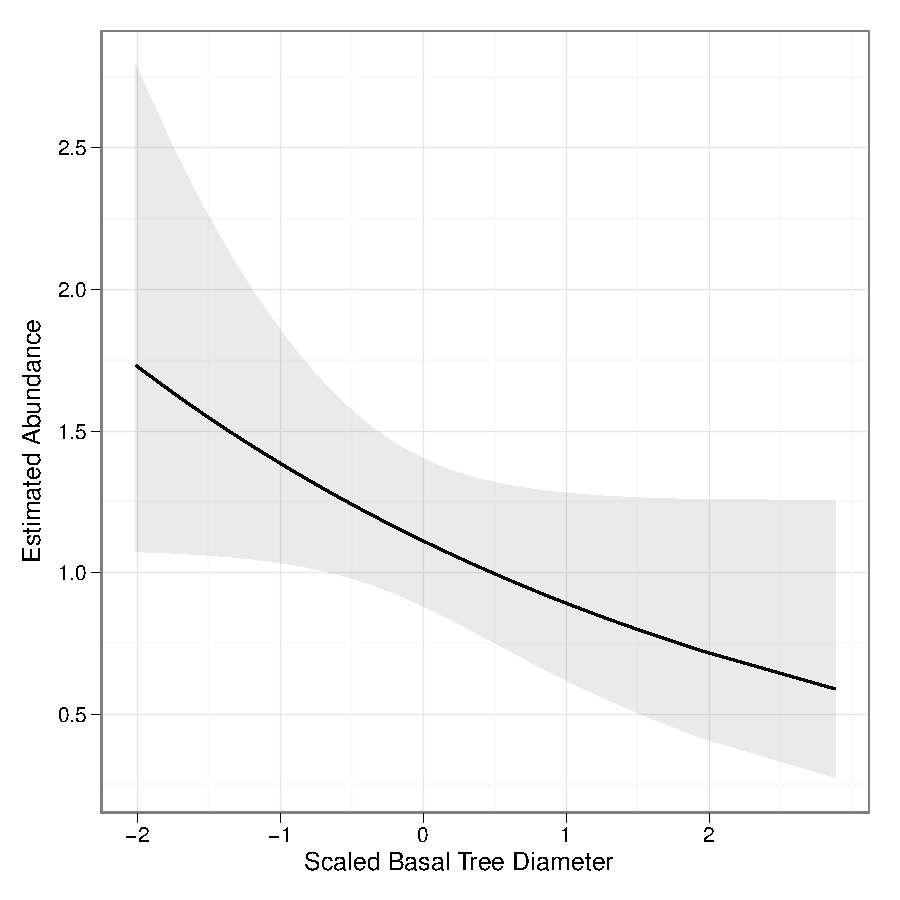
\includegraphics{unmarked-029}
\caption{Examine estimated abundance for Ovenbird removal data.  Band
  is 95\% confidence interval.}
\label{fig:pred}
\end{figure}


It looks like the best model includes only tree basal area as a
predictor of abundance.  We can examine this relationship using
the \code{predict} method (Figure~\ref{fig:pred}).



\begin{Schunk}
\begin{Sinput}
> preddata <- predict(fm3, type = "state", appendData = TRUE)
> library(ggplot2)
> qplot(trba, Predicted, data = preddata, geom = "line", 
+     xlab = "Scaled Basal Tree Area", ylab = "Estimated Abundance") + 
+     geom_ribbon(aes(x = trba, ymin = lower, ymax = upper), 
+         alpha = 0.1) + theme_bw()
\end{Sinput}
\end{Schunk}



\subsubsection{Parametric bootstrap for goodness of fit}

AIC can be used to select the best model in a set, but it does not indicate how well a model fits the data.  To conduct goodness of fit tests, \um\ provides a generic parametric bootstrapping function.  It simulated data from the fitted model and the computes summary information from any specified statistic, with the default being the sum of squared residuals.

%suppress progress report. Probably should add option to argument list too.
\begin{Schunk}
\begin{Sinput}
> set.seed(1234)
> pb <- parboot(fm.oven.1, statistic = SSE, nsim = 20)
\end{Sinput}
\end{Schunk}
\begin{Schunk}
\begin{Sinput}
> pb
\end{Sinput}
\begin{Soutput}
Call: parboot(object = fm.oven.1, statistic = SSE, nsim = 20)

Parametric Bootstrap Statistics:
      t0 mean(t0 - t_B) StdDev(t0 - t_B) Pr(t_B > t0)
SSE 72.2          -3.80             11.6        0.714

t_B quantiles:
    0% 2.5% 25% 50% 75% 97.5% 100%
SSE 50   53  72  77  84    94   97

t0 = Original statistic compuated from data
t_B = Vector of bootstrap samples
\end{Soutput}
\end{Schunk}

\begin{Schunk}
\begin{Sinput}
> plot(pb, main = "Goodness of fit Parametric Bootstrap")
\end{Sinput}
\end{Schunk}

\begin{figure}[h!]
  \centering
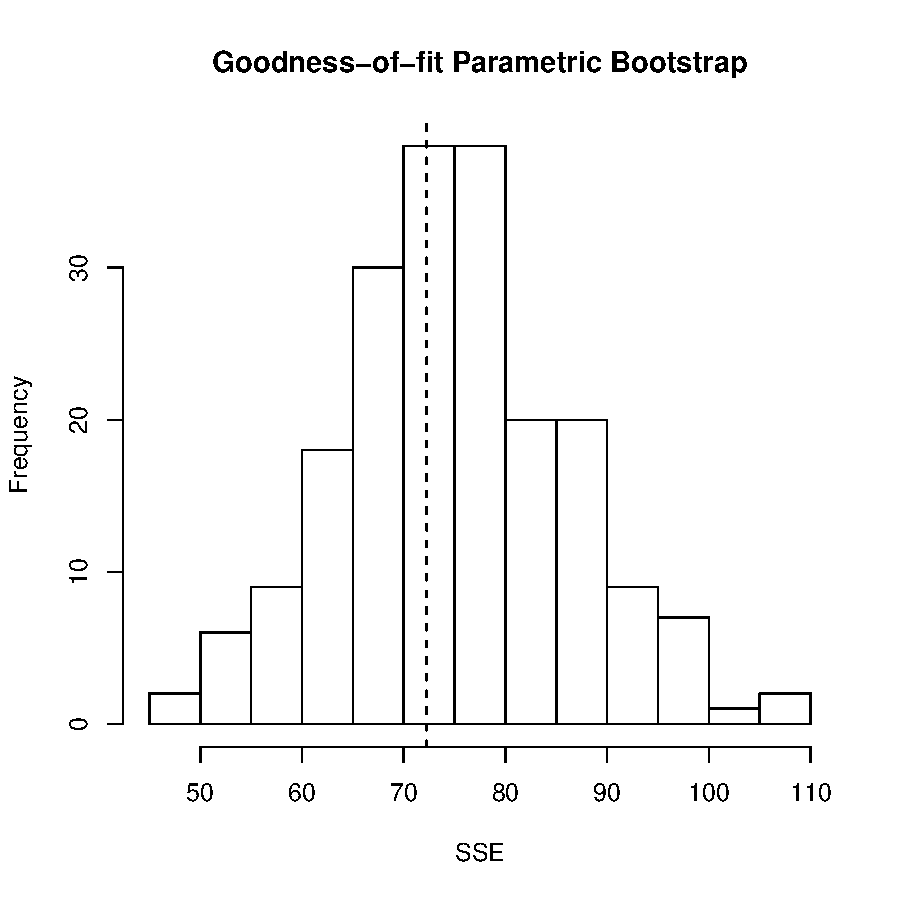
\includegraphics{unmarked-034}
\caption{Graphically assess model fit by parametric bootstrapping
  the sum of squared residuals.  The dashed line is the observed sum
  of squared residuals.}
\label{fig:pb}
\end{figure}


The above call to \code{plot} with a parametric bootstrap object as
the argument produces a useful graphic for assessing goodness of fit
(see Figure~\ref{fig:pb}).  The plot suggests that the model can sufficiently
explain these data.


\section[Future directions for unmarked development]{Future directions for \um\ development}
\label{sec:future-direct-unmark}

\um\ has become a stable and useful platform for the analysis of ecological data, but several areas of development could improve its utility.  First, new models need to be added to cover the range of sampling techniques and population dynamics commonly encountered. Table 3 illustrates the current gaps that need to be filled. In most cases, models to fill these gaps have not been developed so more research is needed.  

\begin{table}[h!] \small
\begin{tabular}{lccc}
\hline
& \multicolumn{3}{c}{Population Dynamics} \\
\cline{2-4} 
Sampling method             & Closed              & Open to movement & Open to demographic processes \\
\hline                            
Occurrence sampling         & \code{occu}         & --               & \code{colext} \\
Repeated counts             & \code{pcount}       & --               & \code{pcountOpen} \\
General multinomial counts  & \code{multinomPois} & \code{gmultmix}  & -- \\
Distance-sampling           & \code{distsamp}     & --               & -- \\
\hline
\end{tabular}
\caption{Models classified by sampling method and population dynamics.}
\label{tab:modelspace}
\end{table}


Second, each of the models in \um\ assumes independence among sites. However, ecologists often use sampling methods such as cluster sampling that induce spatial dependence. Typically, this is done for logistical convenience, but because few methosd are available to account for spatial correlation and imperfect detection probability, the spatial dependence is often ignored.  Rather than this being a weakness of the sampling design, we envision that this dependence can be used as information related to the observation process.  

Finally, Bayesian estimation could be implemented for many of these models.  An important advantage of Bayesian analysis over classical methods is that the latent abundance or occurence variables can be treated as formal parameters.  Thus posterior distriutions could easily be calculated for derived parameters such as the proportion of sites occupied.  Bayesian analysis also would provide a natural framework for incorporating additional sources of random variation. For example, one could model heterogeneity among sites not accounted for by covariates alone.  

\section*{Acknowledgements}

The authors thank Andy Royle of the United States Geological Survey's
Patuxent Wildlife Research Center, who provided initial funding and
inspiration for this work.

\bibliographystyle{jss}
\bibliography{dissertation}

\end{document}
